% !TEX TS-program = XeLaTeX
% use the following command: 
% all document files must be coded in UTF-8
\documentclass{textolivre}
% See more information on the repository: https://github.com/leolca/textolivre

% Metadata
\begin{filecontents*}[overwrite]{article.xmpdata}
    \Title{Barreiras tecnológicas: um fator limitador na acessibilidade das pessoas com deficiência}
    \Author{Marcelo de Santana Porte \sep José Damião Rocha Trindade}
    \Language{pt-BR}
    \Keywords{Acessibilidade \sep Barreiras Tecnológicas \sep Pessoas com Deficiência \sep Meta-análise \sep Revisão de literatura}
    \Journaltitle{Texto Livre}
    \Journalnumber{1983-3652}
    \Volume{14}
    \Issue{3}
    \Firstpage{1}
    \Lastpage{18}
    \Doi{10.35699/1983-3652.2021.32563}

    \setRGBcolorprofile{sRGB_IEC61966-2-1_black_scaled.icc}
            {sRGB_IEC61966-2-1_black_scaled}
            {sRGB IEC61966 v2.1 with black scaling}
            {http://www.color.org}
\end{filecontents*}

\journalname{Texto Livre}
\thevolume{14}
\thenumber{3}
\theyear{2021}
\receiveddate{\DTMdisplaydate{2021}{3}{18}{-1}} % YYYY MM DD
\accepteddate{\DTMdisplaydate{2021}{5}{16}{-1}}
\publisheddate{\DTMdisplaydate{2021}{9}{1}{-1}}
% Corresponding author
\corrauthor{Marcelo de Santana Porte}
% DOI
\articledoi{10.35699/1983-3652.2021.32563}
%\articleid{NNNN} % if the article ID is not the last 5 numbers of its DOI, provide it using \articleid{} commmand
% list of available sesscions in the journal: articles, dossier, reports, essays, reviews, interviews, editorial
\articlesessionname{articles}
% Abbreviated author list for the running footer
\runningauthor{Porte e Trindade}
\sectioneditorname{Daniervelin Pereira}
\layouteditorname{Anna Izabella M. Pereira}


\title{Barreiras tecnológicas: um fator limitador na acessibilidade das pessoas com deficiência}
\othertitle{Technological barriers: a limiting factor in the accessibility of people with disabilities}
% if there is a third language title, add here:
%\othertitle{Artikelvorlage zur Einreichung beim Texto Livre Journal}

\author[1]{Marcelo de Santana Porte~\orcid{0000-0002-7271-6476} \thanks{Email: \url{marcelo_porte@hotmail.com}}}
\author[2]{José Damião Rocha Trindade~\orcid{0000-0002-5788-7517} \thanks{Email: \url{damiao@mail.uft.edu.br}}}

\affil[1]{Universidade Federal do Sul e Sudeste do Pará, Faculdade de Ciências Contábeis, Rondon do Pará, Pará, Brasil.}
\affil[2]{Universidade Federal do Tocantins, Programa de Pós-Graduação em Educação, Palmas, Tocantins, Brasil.}

\addbibresource{article.bib}
% use biber instead of bibtex
% $ biber tl-article-template

% set language of the article
\setdefaultlanguage{portuguese}
\setotherlanguage{english}

% for spanish, use:
%\setdefaultlanguage{spanish}
%\gappto\captionsspanish{\renewcommand{\tablename}{Tabla}} % use 'Tabla' instead of 'Cuadro'
%\AfterEndPreamble{\crefname{table}{tabla}{tablas}\Crefname{table}{Tabla}{Tablas}}

% for languages that use special fonts, you must provide the typeface that will be used
% \setotherlanguage{arabic}
% \newfontfamily\arabicfont[Script=Arabic]{Amiri}
% \newfontfamily\arabicfontsf[Script=Arabic]{Amiri}
% \newfontfamily\arabicfonttt[Script=Arabic]{Amiri}
%
% in the article, to add arabic text use: \textlang{arabic}{ ... }

% for russian text we also need to define fonts with support for Cyrillic script
% \usepackage{fontspec}
% \setotherlanguage{russian}
% \newfontfamily\cyrillicfont{Times New Roman}
% \newfontfamily\cyrillicfontsf{Times New Roman}[Script=Cyrillic]
% \newfontfamily\cyrillicfonttt{Times New Roman}[Script=Cyrillic]
%
% in the text use \begin{russian} ... \end{russian}

% to use emoticons in your manuscript
% https://stackoverflow.com/questions/190145/how-to-insert-emoticons-in-latex/57076064
% using font Symbola, which has full support
% the font may be downloaded at:
% https://dn-works.com/ufas/
% add to preamble:
% \newfontfamily\Symbola{Symbola}
% in the text use:
% {\Symbola }

% reference itens in a descriptive list using their labels instead of numbers
% insert the code below in the preambule:
\makeatletter
\let\orgdescriptionlabel\descriptionlabel
\renewcommand*{\descriptionlabel}[1]{%
  \let\orglabel\label
  \let\label\@gobble
  \phantomsection
  \edef\@currentlabel{#1\unskip}%
  \let\label\orglabel
  \orgdescriptionlabel{#1}%
}
\makeatother
%
% in your document, use as illustraded here:
%\begin{description}
%  \item[first\label{itm1}] this is only an example;
%  % ...  add more items
%\end{description}
 

% custom epigraph - BEGIN 
%%% https://tex.stackexchange.com/questions/193178/specific-epigraph-style
\usepackage{epigraph}
\renewcommand\textflush{flushright}
\makeatletter
\newlength\epitextskip
\pretocmd{\@epitext}{\em}{}{}
\apptocmd{\@epitext}{\em}{}{}
\patchcmd{\epigraph}{\@epitext{#1}\\}{\@epitext{#1}\\[\epitextskip]}{}{}
\makeatother
\setlength\epigraphrule{0pt}
\setlength\epitextskip{0.5ex}
\setlength\epigraphwidth{.7\textwidth}
% custom epigraph - END


% if you use multirows in a table, include the multirow package
\usepackage{multirow}

% add line numbers for submission
%\usepackage{lineno}
%\linenumbers

\begin{document}
\maketitle

\begin{polyabstract}
\begin{abstract}
A presente pesquisa visa avaliar a literatura sobre as barreiras tecnológicas existentes no Brasil direcionadas às Pessoas com Deficiência (PcD). Foram utilizadas as publicações da \emph{SciELO Citation Index} que estão indexadas na base de dados da \emph{Web of Science} desde o ano de 2002, ano de sua indexação, até 2019. Foram realizadas a análise Estatística Textual, a Classificação Hierárquica Descendente e a Análise de Similitude com Nuvem de Palavras de 50 artigos científicos sobre a temática em foco. Os resultados mostram que a literatura sobre as barreiras tecnológicas possui um forte direcionamento para a área da educação, principalmente voltada ao ensino superior, com foco de estudo nos alunos que possuem deficiência visual nas universidades públicas. A literatura sobre barreiras tecnológicas para PcD mostrou que está normalmente associada a outras barreiras de acessibilidade, principalmente as barreiras nas comunicações e informações, sendo raramente encontrada como única variável dos estudos de acessibilidade. Seria relevante expandir os estudos sobre barreiras tecnológicas analisando as principais coleções indexadas na \emph{Web of Science}, o que tornaria possível ter um conhecimento do que vem sendo publicado em periódicos internacionais.

\keywords{Acessibilidade \sep Barreiras tecnológicas \sep Pessoas com deficiência \sep Meta-análise \sep Revisão de literatura}
\end{abstract}

\begin{english}
\begin{abstract}
This research aims to evaluate the literature on the technological barriers in Brazil aimed at People with Disabilities (PwD). SciELO Citation Index publications indexed in the Web of Science database since 2002, were used until 2019. Textual Statistical Analysis, Descending Hierarchical Classification and Similitude Analysis with Cloud of Words of 50 scientific articles on the subject in focus were carried out. The results show that the literature on technological barriers has a strong focus on the area of education, mainly focused on higher education, with a focus on studying students with visual impairment in public universities. The literature on technological barriers for PwD is usually associated with other accessibility barriers, especially barriers in communications and information, and is rarely found as the only variable in accessibility studies. It would be relevant to expand the studies on technological barriers by analyzing the main collections indexed in the Web of Science, in this way it would be possible to have a knowledge of what has been published in international journals.

\keywords{Accessibility \sep Technological barriers \sep Disabled persons \sep Meta-analysis \sep Literature review}
\end{abstract}
\end{english}

% if there is another abstract, insert it here using the same scheme
\end{polyabstract}


\section{Introdução}\label{sec-intro}
Os modelos de negócio na atualidade, ao redor do mundo, têm se transformado com o uso da internet e tecnologias da informação. Antes pequenos negócios, e até mesmo serviços públicos que não se imaginava serem oferecidos por meio de aplicativos, se tornaram uma realidade durante esse período de pandemia do Coronavírus no mundo.

No Brasil, pequenas empresas foram obrigadas a entrarem no e-commerce para não fecharem as portas e optaram por oferecer seus serviços por meio de aplicativos próprios ou se associando às empresas que possuíam serviços já consolidados na internet. No âmbito da educação, instituições de educação básica e superior migraram para ambientes virtuais, sem realizarem um estudo aprofundado das dificuldades tecnológicas, ou até mesmo do possível analfabetismo digital de seus alunos.

Nesse contexto evolutivo da tecnologia, associado à fase pandêmica que o mundo está passando, torna-se necessário dar ênfase aos estudos relacionados às pessoas que sofreram ainda mais com as barreiras tecnológicas, que são as Pessoas com Deficiência (PcD).

Existem muitas variações sobre a forma de realizar um estudo sobre as barreiras tecnológicas direcionadas as PcD. Na literatura, estudos são encontrados com foco em sites universitários europeus \cite{ortega2013} e brasileiros \cite{cantoranipilatti2015}, principalmente no que tange às tecnologias assistivas como os de \textcite{bersch2009, bruno2019, galvaofilho2011, hott2019, martins2012}. Além disso, é válido citar o livro de Romeu Kazumi Sassaki que direciona sua temática à inclusão social das PcD \cite{sassaki2006}, dentre outros.

De acordo com \textcite{vianna2017}, a literatura vem tratando a acessibilidade de forma genérica, devido às suas diferentes dimensões, ou sendo focada especificamente na acessibilidade para PcD física. Por tal motivo, com o presente estudo pretende-se dar ênfase às barreiras tecnológicas, ou seja, esta pesquisa objetiva avaliar a literatura sobre acessibilidade com foco no entendimento de como as barreiras tecnológicas, à luz da Lei Brasileira de Inclusão da Pessoa com Deficiência (Lei no 13.146/2015) \cite{brasil_lei_2015}, estão afetando as PcD.

Este estudo é resultado de uma pesquisa de pós-Doutorado em Educação, realizado na Universidade Federal do Tocantins, e das investigações realizadas pelo Grupo de Estudos e Pesquisas de Currículos Educacionais Grupo de Estudos e Pesquisas de Currículos Educacionais das/para/com Minorias Sociais Nortistas Amazônidas (Gepce/Minorias) do Conselho Nacional de Desenvolvimento Científico e Tecnológico (CNPq).

\section{Método e escopo da revisão}
Trata-se de uma análise de 50 publicações que abordam a temática barreiras tecnológicas, com foco em PcD, indexadas na base de dados \emph{Web of Science}. Tal análise toma como base o processo metodológico realizado por \textcite{porte2018}, que utilizaram os objetivos dos estudos de auditoria para desenvolverem sua pesquisa.

\subsection{A base de dados e os critérios de inclusão e exclusão}
Com o objetivo de avaliar a literatura sobre barreiras tecnológicas no Brasil, foram utilizadas as publicações da \emph{SciELO Citation Index} que estão indexadas na base de dados da \emph{Web of Science}. A \emph{SciELO Citation Index} possui artigos indexados na \emph{Web of Science} desde o ano de 2002.

No primeiro momento, foram selecionadas as publicações que continham o termo “acessibilidade” no campo “tópico” (resumo, título ou palavras-chave). Em seguida, foi realizada a aplicação de um filtro para serem selecionados apenas os artigos específicos da coleção \emph{SciELO} Brasil, até o ano de 2019, gerando um total de 466 documentos a serem analisados.

Na etapa seguinte, todos os estudos foram transferidos para o software EndNote com o objetivo de serem selecionados os estudos que possuíam a temática sobre acessibilidade. A presente análise resultou na exclusão de 342 documentos, haja vista que 333 não corresponderam à temática do presente estudo e nove por serem estudos duplicados, gerando assim uma seleção de 154 artigos sobre acessibilidade a serem consideradas para a análise.

A terceira etapa foi dedicada à seleção dos estudos que possuíam as barreiras tecnológicas como uma das barreiras analisadas em seus estudos. Dessa forma, foi realizada a leitura completa dos 154 estudos à luz da Lei Brasileira de Inclusão da Pessoa com Deficiência (Lei no 13.146/2015) \cite{brasil_lei_2015} com a seleção de 50 artigos que compunham variáveis pertinentes às barreiras tecnológicas experimentadas/encontradas por PcD e posteriormente realizadas as demais análises do estudo com o auxílio do \emph{software IRaMuTeQ}.

\subsection{Elaboração do \emph{corpus} textual e análises aplicadas}
Foi utilizado o estudo de \textcite{marchand2012} para alicerçar a análise léxica e de \emph{keywords} dos objetivos dos 50 artigos utilizados na amostra para a formação do corpus “barreiras tecnológicas”, gerando 1.180 ocorrências, palavras dentro do corpus, das quais apresentaram 477 palavras distintas, sendo 402 formas lematizadas e 264 palavras que ocorreram apenas uma única vez. Ademais, foram identificados 50 segmentos de textos, 364 formas de palavras ativas, 36 formas suplementares, representando uma retenção de 76\% na Classificação Hierárquica Descendente pelo método de Reinert, o que é adequado para a análise a ser realizada \cite{reinert1990}.

Após o processamento da Classificação Hierárquica Descendente (CHD) pelo método de Reinert, foi elaborado o dendrograma das classes (\Cref{fig1}). Obteve-se três classes distintas, o primeiro vértice foi responsável pela criação da Classe 1, com 12 segmentos de textos dos 38 segmentos contidos na CHD, sendo responsável por 31,58\% dos segmentos de todas as classes.

O segundo vértice foi subdividido gerando a Classe 2 e a Classe 3. A Classe 2 associou 11 segmentos de textos, possuindo um total de 28,95\% dos segmentos totais. A Classe 3, maior classe evidenciada com 15 dos 38 segmentos redefinidos, foi responsável por 39,47\% da classe total. Conforme a \Cref{fig1}, adotou-se o símbolo (f) para a frequência individual de cada termo ao longo de uma única classe e o símbolo (N) representa a frequência global de cada termo dentro do \emph{corpus}.

Com esse resultado, foi possível eliminar 24\% de termos considerados não relevantes para o cômputo da revisão de literatura em barreiras tecnológicas para PcD. Os dados na \Cref{fig1} estão apresentados da maior frequência das formas ativas de cada classe para a menor frequência. Optou-se por selecionar apenas as formas ativas, pelo fato de serem mais fidedignas na composição das palavras que compõem os temas centrais dos objetivos dos estudos.

\begin{figure}[htbp]
 \centering
 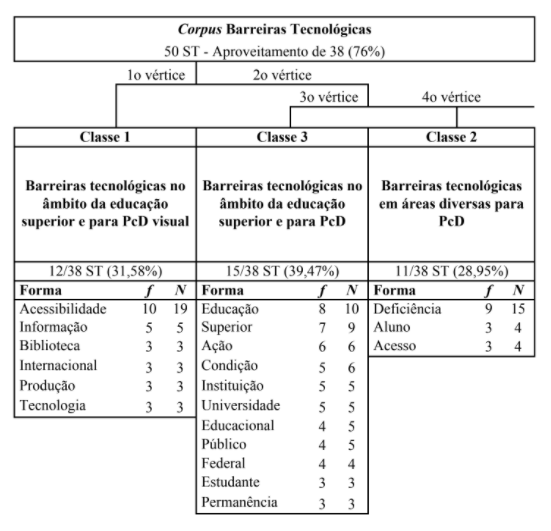
\includegraphics[width=0.75\textwidth]{fig1-32563.png}
 \caption{Dendrograma das classes.}
 \label{fig1}
 \source{Elaboração própria.}
\end{figure}

Para dar continuidade no entendimento do que há na literatura acerca das barreiras tecnológicas que afetam as PcD, optou-se por criar uma Análise de Similitude com Nuvem de Palavras de cada classe de forma separada. Esse procedimento metodológico serve como arcabouço para se entender o que de fato se sabe sobre a temática em foco à luz da Lei Brasileira de Inclusão da Pessoa com Deficiência (Lei no 13.146/2015) \cite{brasil_lei_2015}, de modo semelhante às gerações de classes oriundas dos estudos de \textcite{machado2016, pereira2020}.

Nas próximas seções se apresenta a literatura existente sobre barreiras tecnológicas, com foco para PcD, por meio de uma Análise de Similitude com Nuvem de Palavras de cada classe, por ordem de significância, apresentada no dendrograma de classes (\Cref{fig1}).

\section{Análise e discussões sobre as barreiras tecnológicas}
Esta seção exibe as Estatísticas Textuais e a Análise de Similitude com Nuvem de Palavras de cada classe em um só gráfico.

\subsection{Classe 3 – Barreiras tecnológicas no âmbito da educação superior para PcD}
A Classe 3 “Barreiras tecnológicas no âmbito da educação superior para PcD” obteve a melhor índice de representatividade entre as classes (39,47\%), fornecendo os termos “educação”, “superior”, “ação”, “condição”, “instituição”, “universidade”, “educacional”, “público”, “federal”, “estudante” e “permanência” como os mais representativos entre os 15 Segmentos de Textos (ST) da classe, conforme o dendrograma apresentado na \Cref{fig1}. A \Cref{fig2} apresenta a Análise de Similitude (AS) da Classe 3, com o apoio da Nuvem de Palavras dos termos que melhor compõem a descrição da classe, ou seja, os termos que possuíram uma frequência mínima de três aparições nos objetivos dos artigos.

O \emph{corpus} textual que compõe os estudos de barreiras tecnológicas direcionadas para PcD da Figura 2 é baseado na teoria dos grafos, acoplando as ocorrências das palavras e suas conexões. Observa-se que o resultado da AS (\Cref{fig2}) fornece um destaque para 14 palavras, sendo as 11 destacadas no dendrograma das classes (\Cref{fig1}) com a inserção dos termos “acessibilidade”, “ensino” e “deficiência”. Os resultados apontam três focos dos estudos, 10 deles estão direcionados para a educação superior, três deles para educação básica e dois envolvem pesquisas em temáticas diversas que não estão relacionadas à educação básica ou superior.

\begin{figure}[htbp]
 \centering
 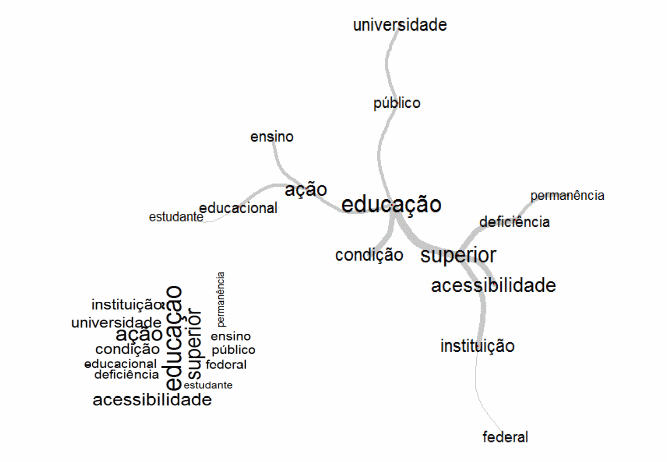
\includegraphics[width=0.95\textwidth]{fig2-32563.png}
 \caption{Análise de Similitude da Classe 3.}
 \label{fig2}
 \source{Elaboração própria.}
\end{figure}

A revisão de literatura apresentou 12 estudos sobre barreiras tecnológicas correlacionadas para a educação superior, oito deles com pesquisas em deficiência não especificada e/ou com abordagem em mais de uma condição \cite{anache2018, branco2019, cantoranipilatti2015, ciantelli2016, garcia2018, melo2018, oliveira2013, siqueira2010} e os outros quatro voltados para PcD visual \cite{carvalho2018, ortega2013, silva+ferreira2017, wataya2006}.

A presente classe possui um maior foco para estudos de barreiras tecnológicas voltadas para estudos no âmbito da educação superior, sendo que suas pesquisas não especificaram a deficiência e/ou que aborda mais que uma deficiência. Seis deles estão direcionados para ações afirmativas \cite{anache2018, ciantelli2016, garcia2018, melo2018, oliveira2013, siqueira2010} que propõem o aumento da acessibilidade no ambiente universitário para alunos PcD, sendo três deles direcionados as suas condições de permanência \cite{anache2018, garcia2018, oliveira2013}, três deles para ações desenvolvidas pelos Núcleos de Acessibilidade das universidades \cite{ciantelli2016, melo2018}, até mesmo o Projeto Incluir \cite{siqueira2010}. Os outros dois, estão voltados para avaliar acessibilidade no âmbito universitário, sendo que um deles, por meio da sua gestão e dos documentos de avaliação do Instituto Nacional de Estudos e Pesquisas Educacionais Anísio Teixeira (INEP) \cite{cantoranipilatti2015}, e o outro, em função da visão dos discentes com deficiência \cite{branco2019}.

De acordo com \textcite{oliveira2013}, os discentes com deficiência não se sentem acolhidos no ambiente universitário, além de possuírem dificuldades na forma proposta de aplicação pedagógica. Tal afirmativa vai ao encontro da visão de \textcite{garcia2018}, pois as autoras ressaltam que um dos problemas significativos nas ações de afirmativas de acessibilidade é o fato de os docentes não estarem preparados para oferecem condições de equidade em suas salas de aula. Vale ressaltar que tudo isso está ligado diretamente ao projeto pedagógico de cada curso, pois, segundo \textcite{anache2018}, os currículos estão engessados pelas barreiras normativas e isso afeta diretamente a possibilidade de se construir um currículo acessível e com o uso de metodologias ativas.

De acordo com \textcite{siqueira2010, ciantelli2016, melo2018}, há necessidade de ampliações das ações de melhorias para as PcD nas universidades brasileiras. Apesar do avanço de normativas legais sobre a acessibilidade no Brasil, continua sendo necessário um maior empenho das ações por parte dos Núcleos de Acessibilidade nas universidades \cite{ciantelli2016} na diminuição das barreiras de acessibilidade para os discentes com deficiência \cite{melo2018}. Afinal, só com um processo de inclusão digno, teremos “um avanço significativo para a instauração de uma sociedade plenamente democrática” \cite[p. 135]{siqueira2010}.

Em seu estudo, \textcite{cantoranipilatti2015} ressaltam que, apesar dos 21 relatórios de avaliação de cursos do INEP afirmarem que a universidade analisada atende de forma suficiente as condições normativas e legais de acessibilidade, os próprios pareceres dos avaliadores vão de encontro com a visão da própria gestão da universidade. De acordo com um dos gestores entrevistados, os problemas financeiros colocam os investimentos em acessibilidade como não prioritários, e, por ser algo comum à maioria das universidades públicas, os avaliadores do INEP acabam sendo complacentes com a situação.

Os dados supracitados corroboram a visão dos discentes avaliada por \textcite{branco2019}. No seu estudo, fica evidenciado que 8, dos 9 entrevistados, que realizam pós-graduação stricto sensu em universidades públicas, possuem tendência de insatisfação ao indicador que avalia as barreiras por insuficiência de recursos pedagógicos e operacionais (computadores, mesas adaptadas, lupa, material em Braile), enquanto o outro respondente se voltou para a insatisfação diante das barreiras que o circundam no dia a dia na universidade.

Apesar de a classe possuir um direcionador para estudos que não especificaram a deficiência e/ou que abordam mais que uma deficiência nas variáveis do seu estudo, a presente classe apresenta estudos que analisaram PcD visual. No primeiro deles pode ser citada a pesquisa realizada por \textcite{wataya2006}, na qual é possível verificar as contribuições da informática no processo de formação educacional para as PcD visual. Os resultados mostram que o uso do leitor de tela DOSVOX e JAWS para o TelEduc permitiram a acessibilidade para PcD visual. Contudo, “a qualidade de contribuição de cada um depende do usuário, no manuseio e decodificação do que é lido em voz alta para eles nas telas visitadas com o apoio dos leitores de tela” \cite[p. 240]{wataya2006}.

Os sites universitários são foco do estudo de \textcite{ortega2013}, no qual foram avaliados vários indicadores de acessibilidade de 75 instituições (públicas e privadas). Em suas considerações finais, é afirmada uma situação positiva de acessibilidade nos sites das universidades, todavia, há aspectos que podem ser melhorados, tais como: “arquitetura e navegação; tratamento e apresentação de recursos de multimídia; e o sistema de busca” \cite[p. 90]{ortega2013}.

\textcite{silva+ferreira2017} aplicaram a técnica de sombreamento em uma universidade pública avaliando a acessibilidade para um aluno com deficiência visual matriculado no curso de educação física. Os resultados mostram que no laboratório da universidade não existem computadores com acessibilidade para PcD visual e o único lugar que possuía um computador assim era no Núcleo de Educação Especial (NEDESP), o qual não ficava no mesmo prédio onde ocorreriam as aulas normalmente, além de ficar a cerda de 20 min de distância de caminhada do Restaurante Universitário e a 10 min do portão de entrada e saída da instituição. As autoras concluem que o uso da técnica de sombreamento permite medir com eficácia a qualidade da acessibilidade para PcD visual.

Ainda com foco na educação superior, a presente classe apresenta o estudo de \textcite{carvalho2018}. Esse estudo avalia o desenvolvimento de um curso de educação no Ambiente Virtual de Aprendizagem (AVA), denominado Sistema Online de Aprendizagem (Solar), alicerçado em tecnologia assistiva, com acessibilidade para PcD visual. O estudo monstra a construção do curso “Hipertensão Arterial: saiba como prevenir”, e devido ao seu sucesso confirmado, as autoras sugerem que a tecnologia assistiva seja utilizada para a promoção da saúde na área da enfermagem.Apesar de o escopo da classe ser direcionado para barreiras tecnológicas na educação superior, ela apresentou dois estudos voltados para a educação básica, sendo que um deles abordou mais que uma deficiência \cite{marins2009} e o outro foi direcionado ao Transtorno do Espectro Autista \cite{santarosa2015}.

\textcite{marins2009} avaliam as políticas públicas voltadas para PcD no que tange a sua inclusão na escola. Foi aplicado um questionário aos gestores da área de Educação Especial das Secretarias Municipais de Educação de seis cidades do estado de São Paulo. Os resultados mostram que apenas duas cidades dispunham de computadores adaptados às necessidades de PcD, sendo comum a todos a falta de outros equipamentos de auxílio para a acessibilidade. Observou-se o não conhecimento dos agentes públicos no que diz respeito à “identificação do número total de alunos que compõem a demanda da Educação Especial" \cite[p. 61]{marins2009} em cada um dos municípios estudados.

O estudo de \textcite{santarosa2015} foca no uso das tecnologias móveis como forma de incluir alunos com Transtorno do Espectro Autista no ambiente de ensino e digital. De acordo com as autoras, “alunos com deficiência estão efetivamente matriculados em escolas públicas brasileiras e, por isso, com direito à utilização de todos os recursos ofertados para mediar o processo de ensino-aprendizagem” \cite[p. 363]{santarosa2015}. Ressalta-se que o laptop utilizado para a modalidade educacional não obteve uma boa utilidade por parte dos pesquisados. Tal fator justificou-se em função da existência de um sistema operacional complexo e com múltiplas escolhas e formas de configurações.

Por fim, a presente classe consta ainda com mais um estudo, sendo este de temáticas diversas (não relacionados à educação básica e à superior) direcionado para mais de uma deficiência \cite{ely2009}. As autoras avaliam a acessibilidade em uma unidade habitacional de hotéis residenciais em Florianópolis/SC. Uma das variáveis analisada foi a utilização de tecnologia assistiva como terminais de computador e telefones com mensagem de texto. Em suas considerações, fica clara a necessidade de se melhorar de forma urgente as condições de acessibilidade nos hotéis residências de Florianópolis.

\subsection{Classe 1 – Barreiras tecnológicas no âmbito da educação superior e para PcD visual}
A Classe 1 “Barreiras tecnológicas a nível da educação superior e para PcD visual” obteve a segunda maior representatividade entre as classes (31,58\%), fornecendo os termos “acessibilidade”, “informação”, “biblioteca”, “internacional”, “produção” e “tecnologia” como os que mais tiveram destaque entre os 12 Segmentos de Textos (ST) da classe, conforme o dendrograma apresentado na \Cref{fig1}.

A \Cref{fig3} apresenta a Análise de Similitude (AS) da Classe 1 com o apoio da Nuvem de Palavras dos termos que melhor compõem a descrição da classe, ou seja, os termos que possuíram uma frequência mínima de três aparições nos objetivos dos artigos.

Observa-se que o resultado da AS (\Cref{fig3}) fornece um destaque para oito palavras, sendo as seis destacadas no dendrograma das classes (\Cref{fig1}) com a inserção dos termos “visual” e “aprendizagem”. Os resultados apontam três focos dos estudos, principalmente direcionados para a educação superior (seis estudos), em pesquisas com temáticas diversas que não estão relacionadas à educação básica e nem à superior (quatro estudos), e, por fim, estudos relacionados à educação básica (dois estudos).

\begin{figure}[htbp]
 \centering
 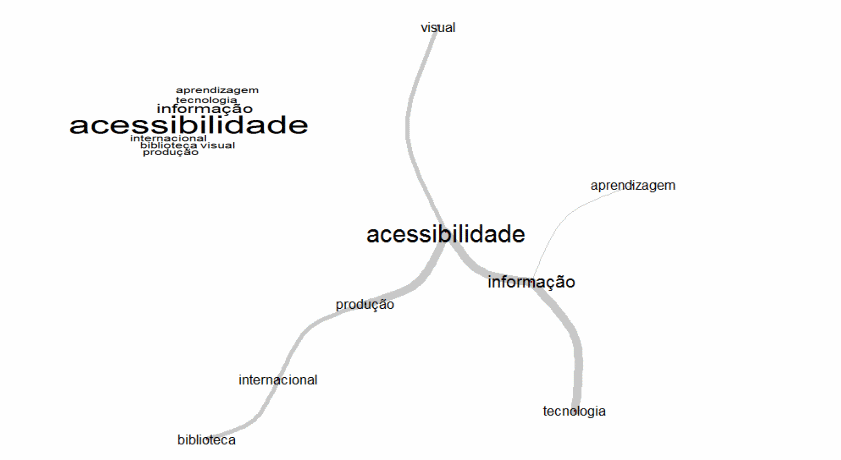
\includegraphics[width=0.95\textwidth]{fig3-32563.png}
 \caption{Análise de Similitude da Classe 1.}
 \label{fig3}
 \source{Elaboração própria.}
\end{figure}

Foram encontrados na literatura seis estudos sobre barreiras tecnológicas correlacionadas à educação superior, três deles possuidores de pesquisas em deficiência não especificada e/ou com abordagem em mais de uma condição \cite{silva+gonzalezgil2017, souza2019, vianna2017}, dois voltados para PcD visual \cite{fialho2012, novelli2014} e um direcionado para PcD auditiva \cite{pivetta2014}.

\textcite{vianna2017} realizaram um estudo bibliométrico com enfoque na acessibilidade para PcD no tocante à tecnologia assistiva na Base de Dados Referencial de Artigos de Periódicos em Ciência da Informação (BRAPCI) e na Library \& Information Science Abstracts (LISA). Os resultados apontam que a temática “deficiência e acessibilidade” é ainda um assunto recente na literatura da Ciência da Informação, possuindo uma característica de desenvolvimento contínuo.

Em estudo também bibliográfico de revisão de literatura sobre a temática acessibilidade de gênero na educação superior, os resultados exibem a participação predominantemente de autoras nos estudos de acessibilidade na educação superior. As autoras ainda afirmam que o presente resultado se justifica pelo fato da existência do interesse das mulheres, muitas vezes, em conteúdos votados ao cuidado e à assistência, enquanto os homens focam em pesquisas direcionadas às áreas de exatas e tecnológicas \cite{silva+gonzalezgil2017}.

Em estudo voltado para a educação superior, \textcite{souza2019} avaliam o nível de acessibilidade do Massive Open Online Courses (MOOCs) disponível na plataforma Lúmina. O estudo foi orientado para a acessibilidade do curso “desconstruindo o racismo na prática”. Os resultados apontam que a plataforma não possui acessibilidade (nas comunicações e informações; e tecnológicas) para todos os seus usuários, gerando dificuldade para PcD \cite{souza2019}.

A literatura apresentou nessa classe a existência de dois estudos voltados para barreiras tecnológicas para PcD visual. O primeiro estudo é o de \textcite{fialho2012}, o qual demonstra a existência de projetos em bibliotecas universitárias, de baixo custo e rápida implementação, direcionados à acessibilidade para PcD visual. Os resultados demonstram que o uso do DOSVOX, distribuição gratuita de material em Braille, e a conversão dos livros físicos para o formato digital pelas bibliotecas fornecem condições de os usuários tornarem-se mais independentes. Contudo, “tão importante quanto o uso de equipamentos e softwares é o preparo dos profissionais para o atendimento aos usuários com deficiência visual” \cite[p. 165]{fialho2012}.

Seguindo as linhas de estudos voltados para bibliotecas universitárias com foco em PcD visual, \textcite{novelli2014} realizaram um estudo com 24 bibliotecas, sendo 7 brasileiras e 17 de universidades estrangeiras. Em suas considerações finais é visto que as bibliotecas investigadas na amostra estão inserindo em seus sites “ferramentas para apoiar os processos de mediação do acesso, busca e aprendizagem do uso de bases de dados, especialmente das bases de dados bibliográficas” \cite[p. 47]{novelli2014}.

Por fim, o último estudo voltado para a educação superior foi o de \textcite{pivetta2014}, o qual possui foco na acessibilidade de um Ambiente Virtual de Aprendizagem (AVA), em especial o Moodle, sendo que voltado para PcD auditiva que possuíam conhecimentos em navegação Web e com nível de pós-graduação. Ao avaliarem de forma automática e humana a disciplina de “capacitação em informática aplicada”, foi percebido que “as avaliações automáticas são eficientes na validação de elementos relativos à codificação, a avaliação humana se mostrou mais adequada nas tarefas relacionadas a aspectos mais subjetivos, como os relacionados à compreensão no ambiente virtual” \cite[p. 159]{pivetta2014}.

Estudos com temáticas diversas (não relacionados à educação básica e superior) também surgiram, com menor expressão, sendo encontrado quatro \cite{alperstedtneto2018, flor2013, hott2019, spolidorio2017} na amostra do estudo para a presente classe. Seguindo a vertente de estudos para PcD auditiva, \textcite{flor2013} realizaram uma pesquisa direcionada para a discussão das recomendações da Web Content Acessibility Guidelines (WCAG) 2.0 no tocante às suas diretrizes de acessibilidade para pessoas surdas. O estudo ratifica que “se por um lado as normas estabelecidas pela WCAG 2.0 favorecem a acessibilidade para PcD no ambiente da web, por outro, a questão da linguagem continua sendo um entrave que distancia o surdo da sua primeira língua (L1 – língua de sinais)” \cite[p. 167]{flor2013}.

Continuando o direcionamento da classe que foca em estudos para PcD visual, \textcite{spolidorio2017} realizou uma pesquisa sobre acessibilidade midiática e a utilização do banco de dados da Media Accessibility Platform (MAP) como meio para o acesso de informações sobre acessibilidade audiovisual brasileira e internacional. Os resultados mostram que o MAP facilita o acesso a informações importantes na área de acessibilidade midiática. “Contudo, muito da produção brasileira, tanto legal quanto acadêmica, ainda precisa ser inserida na plataforma” \cite[p. 343]{spolidorio2017}.

O terceiro estudo em análise foi o de \textcite{hott2019}. Realiza uma reflexão no tocante aos aspectos legais sobre a acessibilidade e a tecnologia assistiva voltados à sensibilização de profissionais de informação a ampliarem seus conhecimentos por meio de uma formação técnico-sistêmica para conseguir atender suas demandas de forma transversal. A pesquisa ratifica que há a necessidade de os profissionais do campo da Ciência da Informação procurarem conhecimentos abrangentes e transversais em prol da acessibilidade em todas as vertentes (física, auditiva, visual, tátil e virtual).

Concluindo o grupo de estudos em temáticas diversas (não direcionados para a educação básica e superior), encontra-se na literatura o estudo de \textcite{alperstedtneto2018}. Sua pesquisa foi direcionada à aplicabilidade da tecnologia para as barreiras de acessibilidade existentes nos ambientes urbanos, transformando cidades comuns em cidades inteligentes. Foi aplicado um questionário para 174 pessoas. No tocante à mobilidade e acessibilidade, os resultados apontam a possibilidade de ser criado “um aplicativo que pudesse ser alimentado pelo usuário e mostrasse rotas para cadeirantes na cidade e a disponibilidade de ônibus” \cite[p. 298]{alperstedtneto2018}. Nas considerações, é apresentado que o aplicativo foi desenvolvido e testado em campo, obtendo resultado positivo de funcionalidade.

Apesar de a presente classe possuir mais características voltadas para estudos da educação superior, a estrutura da classe também trouxe dois estudos direcionados para a área de educação básica, ambos com abordagens para PcD visual \cite{estabel2009, leria2018}.

A pesquisa realizada por \textcite{estabel2009} também mostrou direcionamento para o uso do AVA como meio para realizar treinamentos de professores e bibliotecários com deficiência visual. Em entrevista realizada para os quatro participantes do estudo, ficou evidente que o uso das Tecnologias de Informação e Comunicação existentes no AVA permitiu a integração com seus pares e formadores. Contudo, os participantes do estudo ao utilizarem o recurso para efetuarem a leitura da tela “nas opções “ler todas as mensagens” e da tecla TAB ao longo de todo o texto até encontrar a(s) última(s) mensagem(ns) postada(s), por meio de um sintetizador de voz de teclado” \cite[p. 31]{estabel2009} sentiram-se cansados e carecendo de muita paciência para utilização de tal recurso.

Seguindo ainda em estudo no âmbito da educação básica, \textcite{leria2018} abordam o processo de acessibilidade para PcD visual na realização do Exame Nacional do Ensino Médio (ENEM). São avaliadas as barreiras existentes durante esse processo, sendo proposto um aplicativo denominado ENEM Acessível como solução para os problemas encontrados. De acordo com os dados analisados, o processo atual do ENEM impõe barreiras que limitam o acesso às informações, além de dificultar a compreensão dos quesitos da prova pelos 28 participantes da amostra.

\subsection{Classe 2 – Barreiras tecnológicas em áreas diversas sofridas por PcD}
A Classe 2 “Barreiras tecnológicas em áreas diversas para PcD” obteve a terceira maior representatividade entre as classes do corpus (28,95\%), fornecendo os termos “deficiência”, “aluno” e “acesso” como os mais significativos entre os 11 Segmentos de Textos (ST) da classe, conforme o dendrograma apresentado na \Cref{fig1}.

A \Cref{fig4} apresenta a Análise de Similitude (AS) da Classe 2, com o apoio da Nuvem de Palavras dos termos que melhor compõem a descrição da classe, ou seja, termos que possuíram uma frequência mínima de três aparições nos objetivos dos artigos que compõem a classe.

O resultado da AS (\Cref{fig4}) demonstra uma evidência para seis palavras, sendo três evidenciadas no dendrograma das classes (\Cref{fig1}) com a inclusão dos termos “visual”, “participação” e “acessibilidade”. A classe apresenta um foco para estudos direcionados a áreas distintas da educação básica e da superior com seis estudos. Além disso, encontram-se na classe três estudos para a educação superior e dois para a educação básica.

\begin{figure}[htbp]
 \centering
 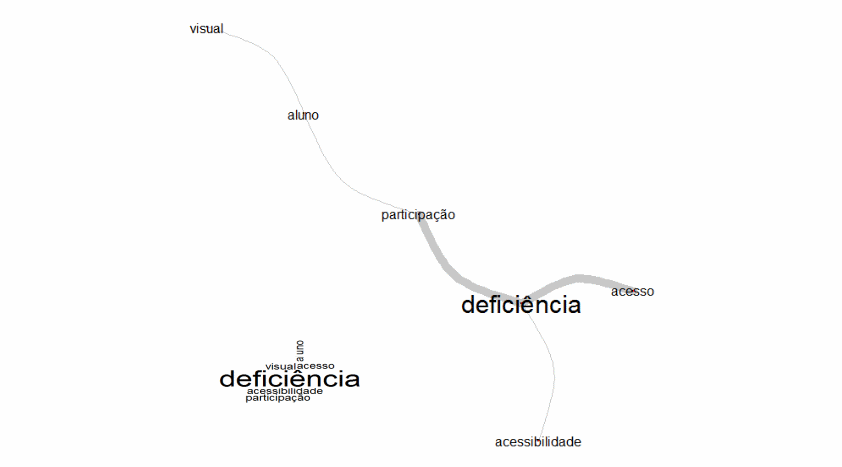
\includegraphics[width=0.95\textwidth]{fig4-32563.png}
 \caption{Análise de Similitude da Classe 2.}
 \label{fig4}
 \source{Elaboração própria.}
\end{figure}

Foram encontrados na literatura seis estudos sobre barreiras tecnológicas correlacionadas a temáticas diversas \cite{amaral2012, cantoranietal2015, freire2009, lima2016, pagliuca2015, silva2015} que não envolvem a área de educação básica e superior. O estudo de \textcite{lima2016} está direcionado para uma análise de acessibilidade de cinco sites específicos para recrutamento e seleção de PcD. O estudo conclui que os sites utilizam informações diferenciadas, no tocante a vaga de emprego, para poderem atrair as PcD. Contudo, mesmo havendo um incentivo de fornecer vagas específicas para PcD, as empresas não estão aptas para receber essas pessoas. Isso ocorre principalmente por não possuírem estrutura física e ferramentas de trabalho que eliminem as barreiras tecnológicas para essas pessoas no âmbito da execução do seu trabalho.

Seguindo a linha dos estudos em sites, \textcite{freire2009} realizaram um estudo longitudinal (1996-2007) para avaliar a evolução da acessibilidade dos sites dos governos estaduais brasileiros. Os resultados mostram que não houve evolução na diminuição das barreiras tecnológicas em seus Portais, gerando assim graves problemas para o cidadão que precisa de informação.

Anos depois, em estudo similar, \textcite{silva2015} realizaram uma análise comparativa da acessibilidade para PcD visual nos Portais Executivos dos estados do Distrito Federal, Bahia, Minas Gerais, Rio de Janeiro, São Paulo, Paraná, Santa Catarina e Rio Grande do Sul. Foram mensurados se os sites apresentavam: página com a descrição dos recursos de acessibilidade, teclas de atalho, barra de acessibilidade e os itens que o compõem, mapa do site, formulário e conteúdo alternativo para imagens. Além disso, foram verificados também os formatos dos documentos disponibilizados no site. Nas suas considerações, destacam que os sites analisados não conseguiram contemplar de maneira plena os indicadores avaliados. Ou seja, os portais executivos analisados não possuíam acessibilidade digital. Ainda conclui que “nada adianta um país afirmar que se preocupa com a situação das PcD, se não implementa as condições necessárias para que elas possam se afirmar como verdadeiros sujeitos de direito” \cite[p. 334]{silva2015}.

Seguindo na vertente de políticas públicas inclusivas, é possível ver na literatura o estudo de \textcite{pagliuca2015}, que realizam uma pesquisa com 120 PcD, divididas de igual forma (40 visual, 40 auditiva e 40 física). Os resultados mostram que, apesar de as PcD visual considerarem positivas as políticas públicas, e haver pontos positivos para ações inclusivas (PcD visual) e ações de acessibilidade física (PcD física) sendo que em menor número, todos concordam que as políticas públicas não cumprem o mandato de inclusão na educação e na saúde.

Corroborando essa afirmativa, pode ser citado o estudo de \textcite{amaral2012}, no qual é dada ênfase na necessidade de se dar atenção para o idoso e a necessidade da reorganização dos serviços de saúde. O seu estudo analisou as variáveis que estão associadas às dificuldades encontradas por 244 idosos com deficiência ao acessar os serviços de saúde em João Pessoa/PB. Os resultados comprovaram que 73,8\% dos idosos pesquisados necessitam de algum tipo de tecnologia assistiva. Os idosos da amostra possuíam deficiência mental, visual, física, auditiva, múltipla e de mobilidade reduzida.

Por fim, o estudo de \textcite{cantoranietal2015} analisou documentos direcionados ao WHOQOL-DIS como instrumento fornecedor de qualidade de vida para PcD. Os resultados evidenciam que o instrumento WHOQOL-DIS não apresenta questões que mesuram as adaptações ambientais realizadas devido às suas limitações, e nem indicadores para averiguar se as barreiras físicas existentes no seu cotidiano estão influenciando a sua vida no dia a dia. Conclui-se de forma incisiva que “a não inclusão dessas questões desconsidera o fato da acessibilidade e da autonomia estarem conceitualmente relacionadas à efetivação ou não da deficiência” \cite[p. 423]{cantoranietal2015}.

Apesar de a presente classe possuir um perfil direcionado para estudos fora do ambiente educacional, a literatura apresentou três estudos voltados para a educação superior \cite{camargo2008, gesser2017, nogueira2018} e dois para a educação básica \cite{kraemer2018, oliva2016}. Em relação aos problemas que ocorrem no âmbito da educação, em particular a educação superior, há o estudo de \textcite{camargo2008}. Nele são verificadas as barreiras que dois alunos com deficiência visual enfrentam ao passar pela aula de óptica, conteúdo da disciplina de Física. Um deles perdeu a visão ao longo da vida e o outro aluno é cego desde o seu nascimento. Os resultados apresentam que das 101 barreiras comunicacionais encontradas pelos alunos no estudo, cerca de 41,6\% delas são comuns aos dois alunos estudados. Para um melhor aproveitamento do aluno, seria necessário a utilização recursos tecnológicos para diminuição dessa barreira.

\textcite{nogueira2018} analisaram em seu estudo o Programa Incluir do Ministério da Educação, direcionados a 55 Instituições Federais de Ensino Superior (IFES) com Núcleos de acessibilidade. Foram entrevistados os coordenadores com o objetivo de saber a atuação do curso de graduação em terapia ocupacional no Programa Incluir. Os resultados apresentam que apenas três dos 14 cursos ativos possuíam terapeutas ocupacionais como coordenadoras dos Núcleos de acessibilidade. Ficou evidenciada a existência de unidades curriculares específicas voltadas para a tecnologia assistiva na composição curricular de todos os cursos. Ressalta-se que temas como educação e deficiência (em todos os níveis de escolaridade) deveriam fazer parte da formação inicial dos alunos de terapia ocupacional, fazendo com que eles refletissem, juntamente com os docentes, sobre formas de aumentar as contribuições dos terapeutas ocupacionais no processo de inclusão de PcD.

Seguindo uma abordagem de teorias feministas, \textcite{gesser2017} realizaram um estudo de revisão de literatura voltado para os problemas de acesso e permanência de discentes no ensino superior, em especial as PcD física e visual. Os autores afirmam que as universidades são responsáveis pelo provimento de tecnologia assistiva aos discentes e que deveria haver disponibilidade de computadores com programas de leitor de tela para a inclusão digital dos mesmos. Além disso, \textcite[p. 151]{gesser2017} ressaltam a necessidade de “recursos tecnológicos como lupas eletrônicas, \emph{thermoforming} e impressora 3D” para promover a acessibilidade informacional para o discente.

Seguindo o foco de estudo em educação, sendo que dessa vez direcionado à educação básica, a literatura apresentou dois estudos que abordaram a participação e o aprendizado do aluno no âmbito escolar. O primeiro estudo é o de \textcite{oliva2016}, no qual são analisados a qualidade do processo de inclusão escolar e as barreiras para uma aluna com deficiência visual. Um fato que chamou a atenção nos resultados do estudo é que a aluna pesquisada não questionava o fato de a escola não possuir nas aulas de informática materiais adequados, como Dosvox e teclado em braile, para realização da sua inclusão digital. As considerações do estudo são contundentes ao afirmar que, infelizmente, a escola pesquisada não implementava políticas de inclusão, dificultando cada vez mais o processo de desenvolvimento de práticas inclusivas no âmbito da educação básica.

Por fim, em um estudo teórico, \textcite{kraemer2018} analisaram as leis e políticas públicas criadas a partir de 2000 que envolvem a temática de inclusão de PcD. Os resultados nos documentos analisados mostram ações importantes que objetivaram o acesso, a participação, desenvolvimento e aprendizagem na escola, tais como: Implementação de salas com recursos multifuncionais; o Programa Escola Acessível; o Transporte Escola Acessível; o Pronatec; o Programa Incluir e o Programa Viver Sem Limite. As autoras ressaltam que “a governabilidade biopolítica na qual se inscreve a inclusão escolar tem na acessibilidade sua principal estratégia para efetivar uma política econômica e social que conte com a participação de todos, ainda que isso não capture a todos” \cite[p. 561]{kraemer2018}.

Vale ressaltar que o Dendrograma das Classes (\Cref{fig1}) pré-selecionou 38 dos 50 estudos da amostra. Os demais 12 estudos não selecionados para a formação das classes foram eliminados das análises sem prejuízo para o entendimento da revisão de literatura analisada. De acordo com os estudos não selecionados:

\begin{itemize}
    \item sete deles estão relacionados às barreiras tecnológicas em temáticas diversas \cite{barbosa2018, borges2018, carvalho2003, oliveira2015, soares2016, souza2018, souza2016};
    \item três para a educação básica \cite{bruno2019, petroni2018, santarosa2012};
    \item dois para a educação superior \cite{flor2015, lazzarin2015};
    \item cinco estão direcionados para a deficiência visual \cite{borges2018, bruno2019, lazzarin2015, oliveira2015, souza2018};
    \item quatro abordam a deficiência auditiva \cite{barbosa2018, flor2015, soares2016, souza2016};
    \item dois possuem deficiência não especificada e/ou com abordagem em mais de uma condição \cite{carvalho2003, santarosa2012};
    \item um estudo é direcionado à deficiência física \cite{petroni2018}.
\end{itemize}

\section{Discussão dos resultados}
De acordo com a Lei Brasileira de Inclusão (Lei nº 13.146/2015) \cite{brasil_lei_2015}, a sociedade está sujeita às seguintes barreiras: urbanísticas; arquitetônicas; nos transportes; nas comunicações e informações; atitudinais; e tecnológicas. Os resultados assinalam que melhorias vêm sendo realizadas para a diminuição das barreiras tecnológicas para as PcD, sobretudo pela evolução legal, como a criação do decreto que promulga a Convenção Internacional sobre os direitos das pessoas com deficiência (Lei nº 6.949/2009) \cite{brasil_lei_2009}, e de políticas públicas no cenário brasileiro ao longo dos últimos anos.

O foco do presente estudo está direcionado às barreiras tecnológicas. Por tal motivo, foi percebido nos resultados analisados que poucos são os estudos que estudam unicamente essa barreira como variável de estudo. Podem ser citados os estudos de \textcite{vianna2017, cantoranietal2015}. Normalmente, os estudos de barreiras tecnológicas estão associados às barreiras nas comunicações e informações, como pode ser visto nos estudos de \textcite{santarosa2015, camargo2008}.

A literatura sobre barreiras tecnológicas possui um forte direcionamento para a área da educação superior, como apresentado pelos resultados das Classes 1 e 3. A universidade pública é fonte principal dos estudos, com temas que envolvem as ações de políticas afirmativas \cite{ciantelli2016, melo2018, oliveira2013, siqueira2010}, de educação inclusiva para os estudantes \cite{branco2019, marins2009}, principalmente as relacionadas ao processo de permanência na universidade \cite{anache2018, garcia2018, oliveira2013} e a acessibilidade de bibliotecas universitárias \cite{souza2019}.

Estudos voltados para as áreas que estão fora do ambiente da educação básica e superior mostraram-se fortes na literatura, gerando a Classe 2. São eles estudos voltados para o funcionamento e a acessibilidade de sites governamentais \cite{freire2009, oliveira2013} e de recrutamento e seleção \cite{lima2016}.

No tocante à deficiência que está sendo usada como variável nos estudos sobre barreiras tecnológicas, a literatura é contundente em demostrar que a deficiência visual é a mais evidenciada. O uso da técnica de sombreamento auxilia pesquisadores na evidência de problemas que PcD visual experimentam com as barreiras tecnológicas em vários momentos do seu cotidiano \cite{silva+ferreira2017}.

A literatura apresentou também estudos específicos para PcD auditiva, mas em menor proporção. De acordo com \textcite{flor2013}, as entidades, públicas e privadas, devem melhorar a acessibilidade das pessoas surdas no ambiente da web. Para avaliar a acessibilidade é necessário que sejam utilizadas, concomitantemente, as técnicas de avaliação automática e humana nos ambientes que envolvam o uso do computador como meio de transmissão da informação \cite{pivetta2014}.

A grande maioria dos estudos sobre barreiras tecnológicas utilizam mais de uma deficiência como variável ou não especificaram o tipo da deficiência em si. O aumento do número de PcD na sociedade, e, por conseguinte, o número de matriculados no ambiente educacional, são desafios importantes, para os quais a gestão da informação deve ficar atenta, para que haja um processo de inclusão social e escolar \cite{vianna2017}. Isso porque, “a partir da política de inclusão, a diversidade apresenta-se como elemento para o convívio social e para os processos de ensino e aprendizagem” \cite[p. 560]{kraemer2018}.

Apesar das barreiras tecnológicas do ensino básico não terem sido uma classe predominante entre as três classes geradas de acessibilidade no estudo, ela é relevante para a temática na literatura. Apesar dos holofotes serem direcionados para a educação superior, as barreiras tecnológicas para PcD na educação básica são muito comuns e estão muito longe de ser eliminadas. Para que ocorram melhorias no processo de inclusão no ambiente da educação básica é necessário que sejam criados padrões de acessibilidade e de usabilidade de serviços, como de produtos, nos ambientes educacionais \cite{souza2019}. Além dos problemas durante toda a educação básica, o aluno com deficiência possui dificuldade para ser aprovado no processo seletivo na universidade. De acordo com \textcite{leria2018}, o uso da tecnologia diminui os problemas para esse cenário, mas não fornece totalmente uma acessibilidade para o estudante.

\section{Considerações finais}
Pode-se concluir que a literatura sobre barreiras de acesso à tecnologia está direcionada mais para a área de educação, principalmente a relacionada à educação superior pública. Há uma necessidade de mais estudos específicos sobre barreiras tecnológicas, como única variável estudada, dissociando-as de outras barreiras de acessibilidade. A literatura mostra que a tecnologia assistiva tem se tornado um elemento-chave para a inclusão e independência das PcD.

Outro fator importante a ser considerado é que há poucos estudos específicos apresentando a realidade das PcD auditiva, como também as PcD física, no tocante às barreiras tecnológicas. É comum encontrar estudos com variáveis que mensurem as barreiras tecnológicas associada aos estudos sobre as barreiras nas comunicações e informações, ou quando fazem parte de um conjunto de indicadores que objetivam analisar várias barreiras de acessibilidade principalmente para PcD.

Ambiciona-se poder, com este estudo, incentivar o Núcleo de Inclusão e Acessibilidade do Deficiente (NIADI) da Universidade Federal do Tocantins (UFT) a adicionar a barreira tecnológica como umas das barreiras de acessibilidade a serem trabalhadas pelo Núcleo na UFT.

Mediante os resultados aqui encontrados, sugere-se que sejam realizadas pesquisas que mensurem as dificuldades para PcD no âmbito público em comparação com o privado, de preferência para os discentes do mesmo curso, durante o período da pandemia do Coronavírus, quando realizaram seus estudos de forma remota.

Um fator limitante do estudo foi utilizar a base de dados da \emph{Web of Science}, em especial as publicações indexadas na SciELO Brasil. Seria relevante expandir os estudos sobre barreiras tecnológicas analisando as principais coleções indexadas na \emph{Web of Science}, o que permitiria ter um conhecimento do que vem sendo publicado em periódicos internacionais.

Outro delimitador do estudo foi a utilização dos sujeitos em segundo plano, dando ênfase às barreiras e deficiências encontradas na amostra do estudo, não sendo analisados seus sentimentos.



\printbibliography\label{sec-bib}
% if the text is not in Portuguese, it might be necessary to use the code below instead to print the correct ABNT abbreviations [s.n.], [s.l.] 
%\begin{portuguese}
%\printbibliography[title={Bibliography}]
%\end{portuguese}

%full list: conceptualization,datacuration,formalanalysis,funding,investigation,methodology,projadm,resources,software,supervision,validation,visualization,writing,review
\begin{contributors}[sec-contributors]
\authorcontribution{Marcelo de Santana Porte}[conceptualization,datacuration,formalanalysis,investigation,methodology,projadm,software,validation,writing]
\authorcontribution{José Damião Rocha Trindade}[supervision]
\end{contributors}


\end{document}
